%!TEX root=paper.tex

\section{The Need for Active Management of Processor Timing Margin}
\label{sec:motivation}

This section explains the basics of microprocessor's timing margin, and motivates why active management of timing margin is necessary to improve power efficiency. This section first goes over the necessity of timing margin in modern microprocessors. Then it enumerates the main components involved in timing margin. We end this section with a brief discussion of the working mechanism of active timing margin.

\subsection{The Importance of Timing Margin in Modern Microprocessors}

In the abstract form, general-purpose microprocessors are state machines that follows the von-Neumann architecture. In practice, microprocessors must be implemented in a physical form to perform the actual computation, be it add, multiply, store, or others. The physical implementation dates back to an early mechanical form as the Babbage Engine in the 1800s, and has evolved a long way to today's highly efficient electronic form as CMOS transistors. Whatever microprocessor's physical form of implementation is, they must be made and delivered with reliability guarantee, as any other human-engineered, physical instance that operate in the presence of uncertainty. Uncertainty exists because human do not have perfect control in the manufacturing and operating process. Uncertainty can be systematically biased, or purely random. Either way, it must be taken into account in a microprocessor's design, manufacturing and testing.

Modern processor's micro-architecture is pipelined for higher performance. All pipeline stages have the same time duration to complete their computing tasks, synchronized by a global clock. In each pipeline stage, circuits constructed by CMOS transistors take some time to switch and then produce a stable output electric level. In an ideal world, the circuit's switch time can be calculated using CMOS device's charge and discharge time formula given a particular supply voltage and transistor size, and pipeline cycle time should be equal to the circuit switch time, assuming all pipeline stage have the same switch time. However, in the real world, circuit switch time can have lots of uncertainty caused by, for instance, imperfect transistor size during manufacturing, transistor performance variation due to heating, or imperfection in supply voltage, etc. The uncertainty could make circuits complete their jobs faster, or slower than the time duration calculated by theoretical formulas. To assure all circuits have plenty of time to get their jobs completed, pipeline cycle time is always longer than the theoretical circuity switch time, the added time duration in clock cycle is called \textit{timing margin}, as illustrated in~\Fig{fig:timing-margin}.

A good analogy of microprocessor pipeline's timing margin in everyday life is the relationship between cars and lanes. In an ideal world, a lane would have the same width as a car because car would strictly obey the orbits of the lane. Yet, in the real world, lanes are always (much) wider than cars because cars often deviate from lane orbits by some error, or uncertainty. The deviation uncertainty may be caused by human driver's improvisation, or the inherent control error of the vehicle (e.g., a mismatch between the left and right tires). The extra space between a lane and a car allows the car to correct itself and stay on track. The extra room between lane width and car width works just like how pipeline timing margin protects against circuit's timing uncertainty.

\begin{figure*}[t]
\centering
\subfloat[Static timing margin.] {
  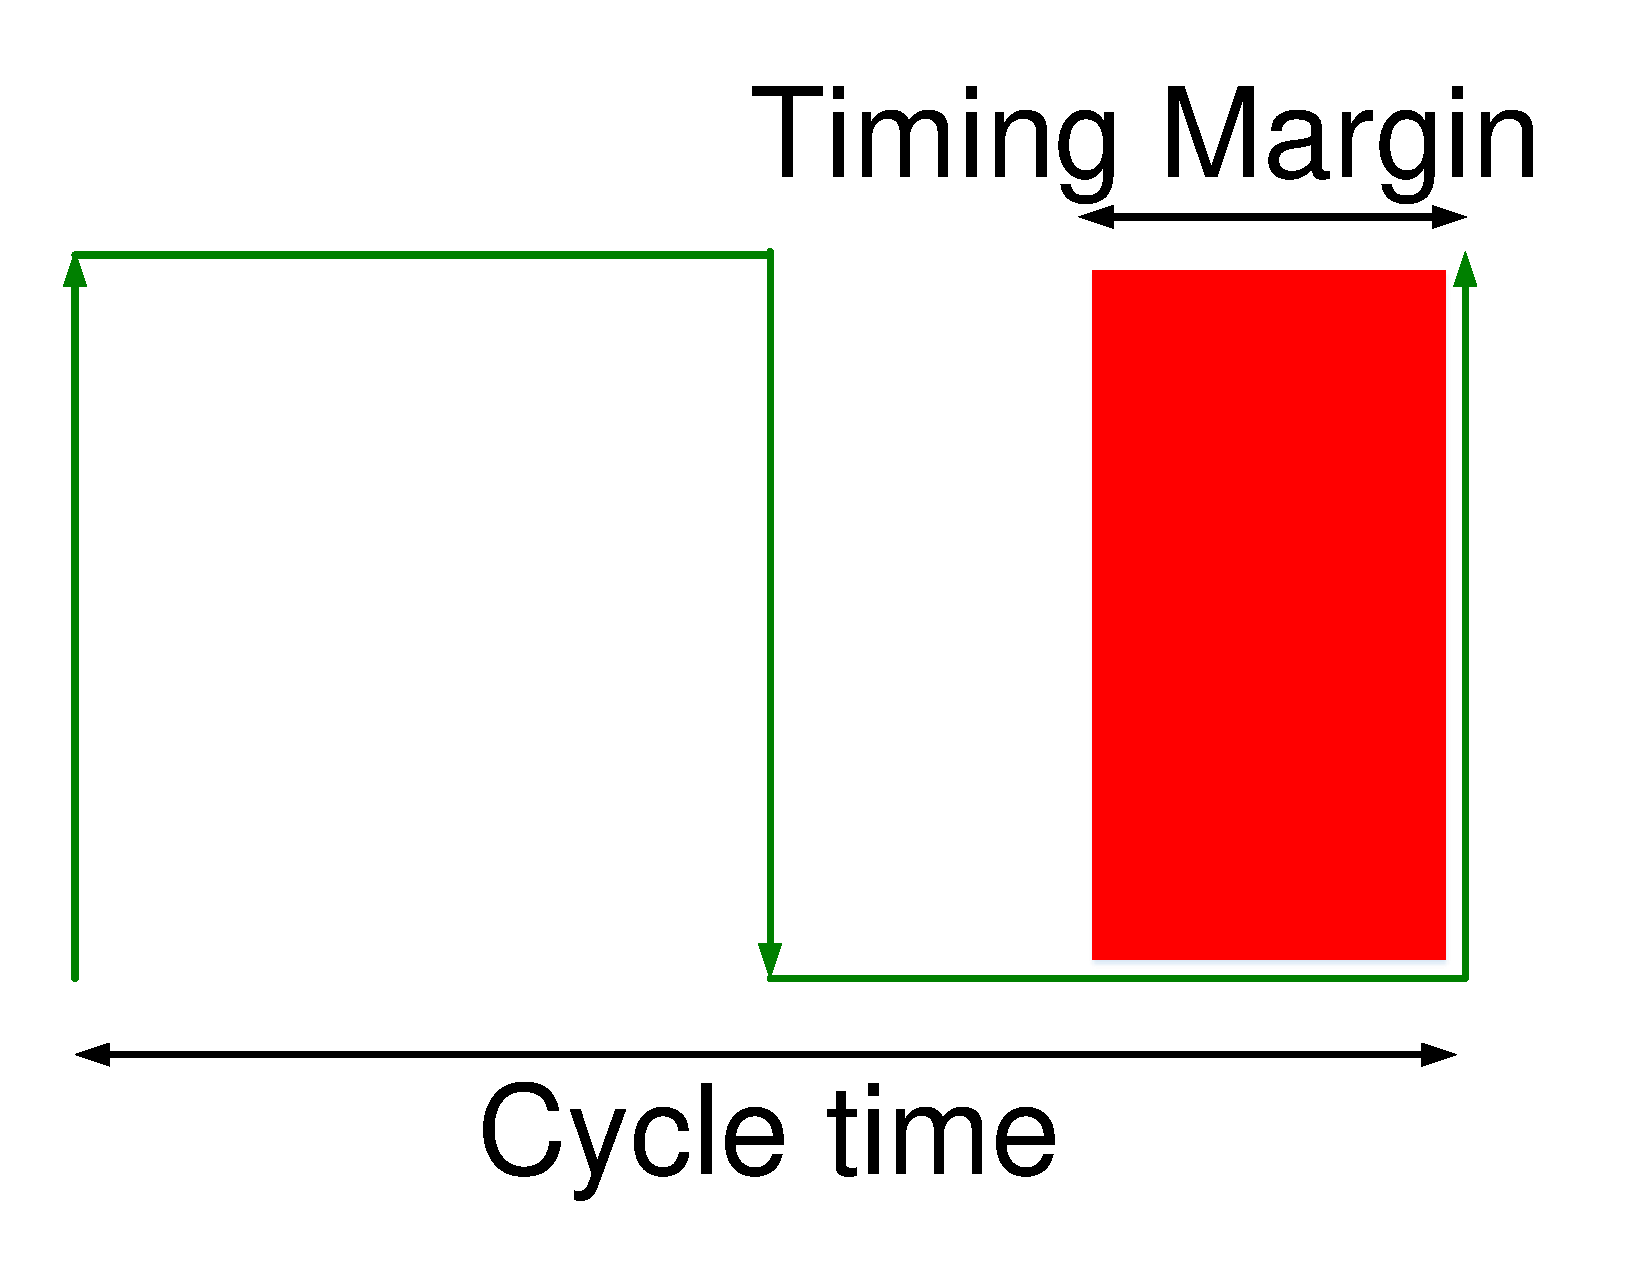
\includegraphics[trim=0 0 0 0,clip,width=.25\linewidth]{graphs/timing-margin.pdf}
  \label{fig:timing-margin} 
}
\hfill
\subfloat[Voltage guardband.] {
  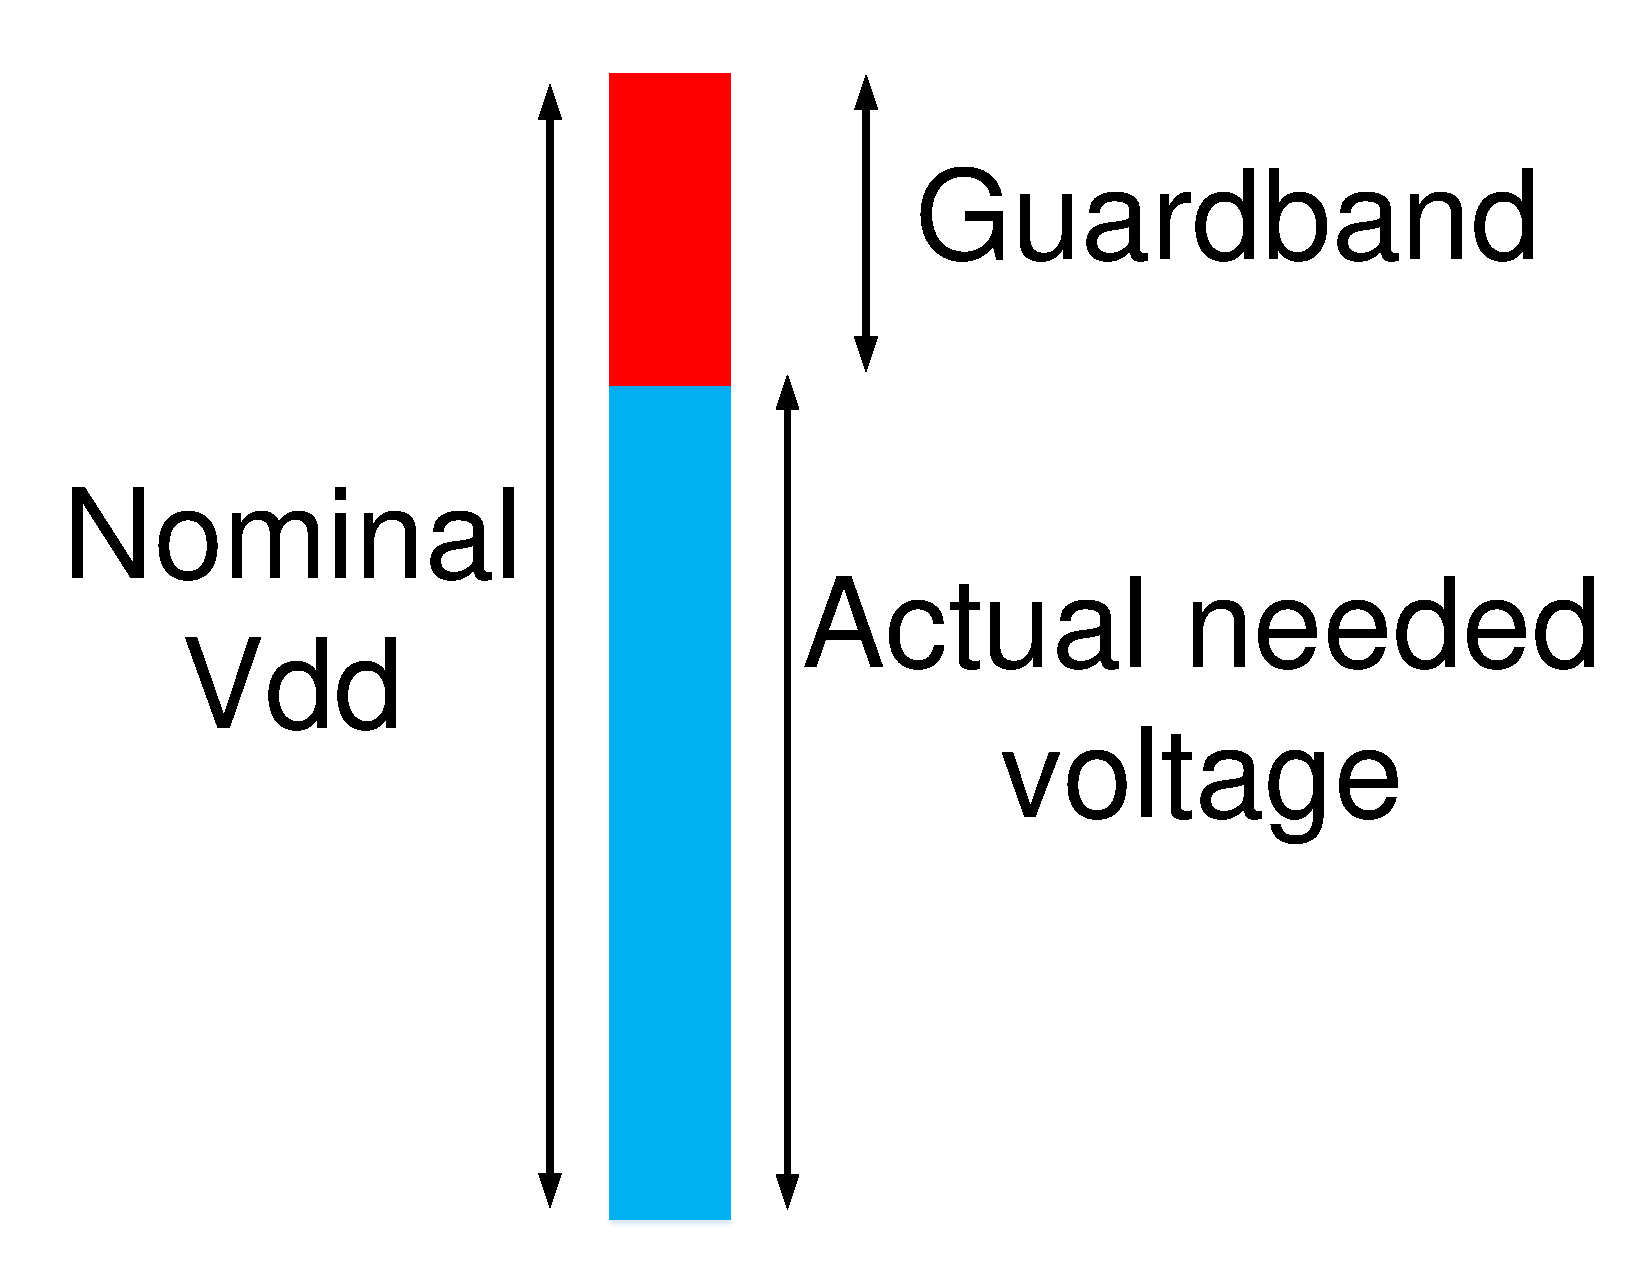
\includegraphics[trim=0 0 30 0,clip,width=.25\linewidth]{graphs/voltage-guardband.pdf}
  \label{fig:voltage-guardband} 
}
\hfill
\subfloat[Active timing margin.] {
  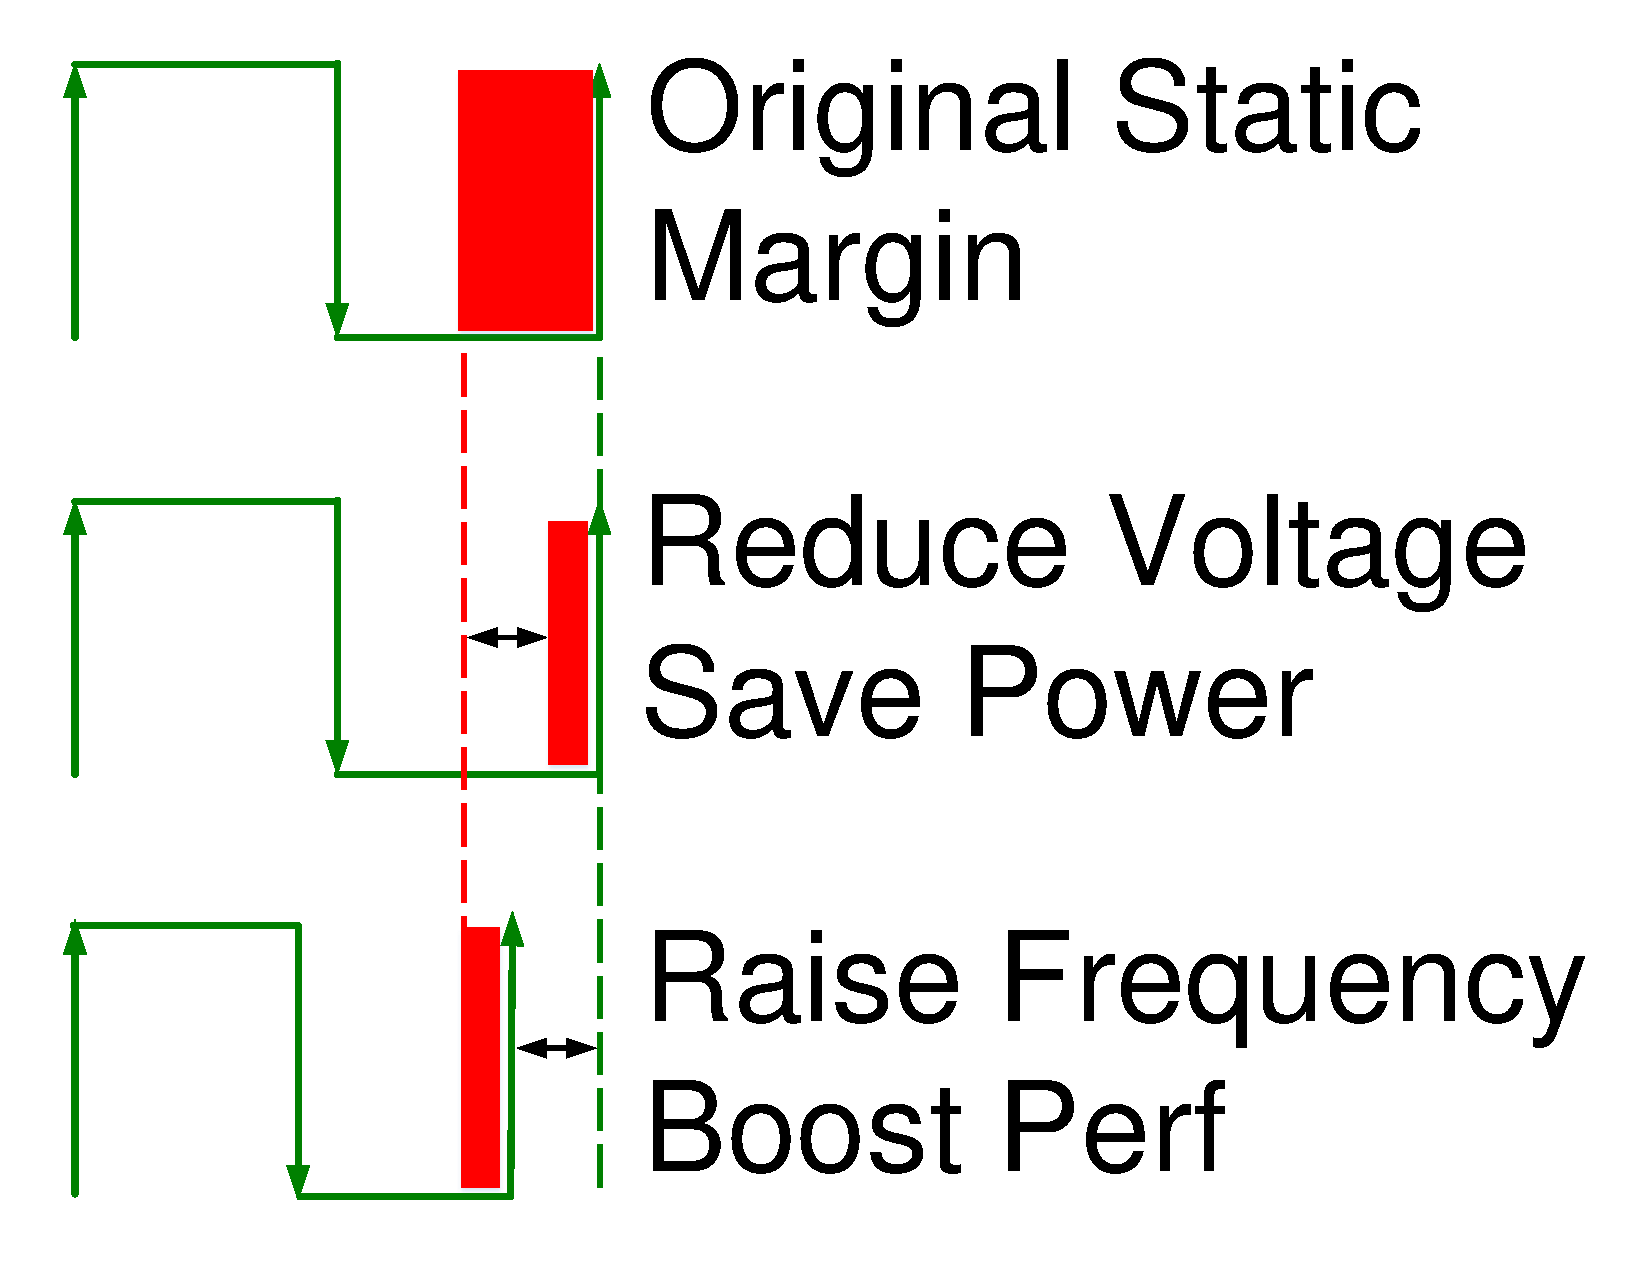
\includegraphics[trim=0 0 0 0,clip,width=.25\linewidth]{graphs/adaptive-margin.pdf}
  \label{fig:adaptive-margin} 
}
\caption{Timing margin ensures reliability by creating extra room in pipeline's clock cycle time. It can be delivered by providing extra voltage, known as the voltage guardband. Active timing margin improves from conventional static margin with tighter clock cycle by overclocking or undervolting.}
\end{figure*}

Failing to take circuity's performance uncertainty into account can lead to the microprocessor malfunction. One good example is the rowhammer problem discovered in DRAM chips recently~\cite{kim2014flipping}. In DRAM chips, stressing one row can cause the row's adjacent cells to leak charge quicker than usual, and eventually causes a bit flip which may have serious repercussions. To protect against this situation, DRAMs need to provide ample headroom to tolerate the uncertainty in a cell's charge leakage time, such as by refreshing cells quicker which is a form of timing margin. Though DRAM is not exactly the same as a microprocessor, this case illustrates the importance of timing margin in CMOS chips.

\subsection{Major Consumers of Microprocessor's Pipeline Timing Margin}
\label{sec:motivation:perf}

Timing margin can be implemented as tuning supply voltage slightly higher, which makes circuits operator faster and thus leaving some timing slack, or tuning the frequency slightly slower, which makes cycle time longer. These two methods are equivalent to each other. The former approach is widely known as \textit{voltage guardband} as described in \Fig{fig:voltage-guardband}. We explore both methods in this thesis.

In today's CMOS chips, the amount of timing margin needed to ensure microprocessor reliability is often excessively high because of the various sources of timing uncertainty. Prior art has tried to quantify the magnitude voltage guardband on GPUs. In~\cite{leng2015safe} researchers report around 20\% voltage guardband from commercial products, which can amount to more than 25\% power and energy wastage. The wastage is significant not only because of the power and energy it consumes, but also because today's microprocessors are inherently power limited, and wasting power means limiting processor performance. Therefore it is imperative that we investigate what leads to timing uncertainty and consumes timing margin. 

\paragraph{Temperature variation} is one important source of timing uncertainty. When temperature changes, transistor performance varies because temperature variation alters the activity level of the particles in the semiconductor material, which changes transistor switch speed and circuit completion time.In practice, processor temperature variation is unavoidable because during workload run the charge and discharge of semiconductor transistors inevitably raises temperature. Depending on workload intensity, the temperature profile of the chip varies temporarily and spatially, affecting circuit timing. To tolerate timing uncertainty caused by temperature variation, margin must be added in the cycle time. In \label{sec:tistate} we perform an in-depth study on how temperature affects timing uncertainty and device architecture and system level mechanisms to combat against it.

\paragraph{Voltage variation} is a complex source of timing uncertainty. It is caused by the interaction between the parasitics of the power delivery subsystem of a microprocessor and the varying power draw under workload stress. \Fig{fig:pdn-model} gives an overview of the physical mechanism of voltage variation.

\begin{figure*}[t!]
  \centering
  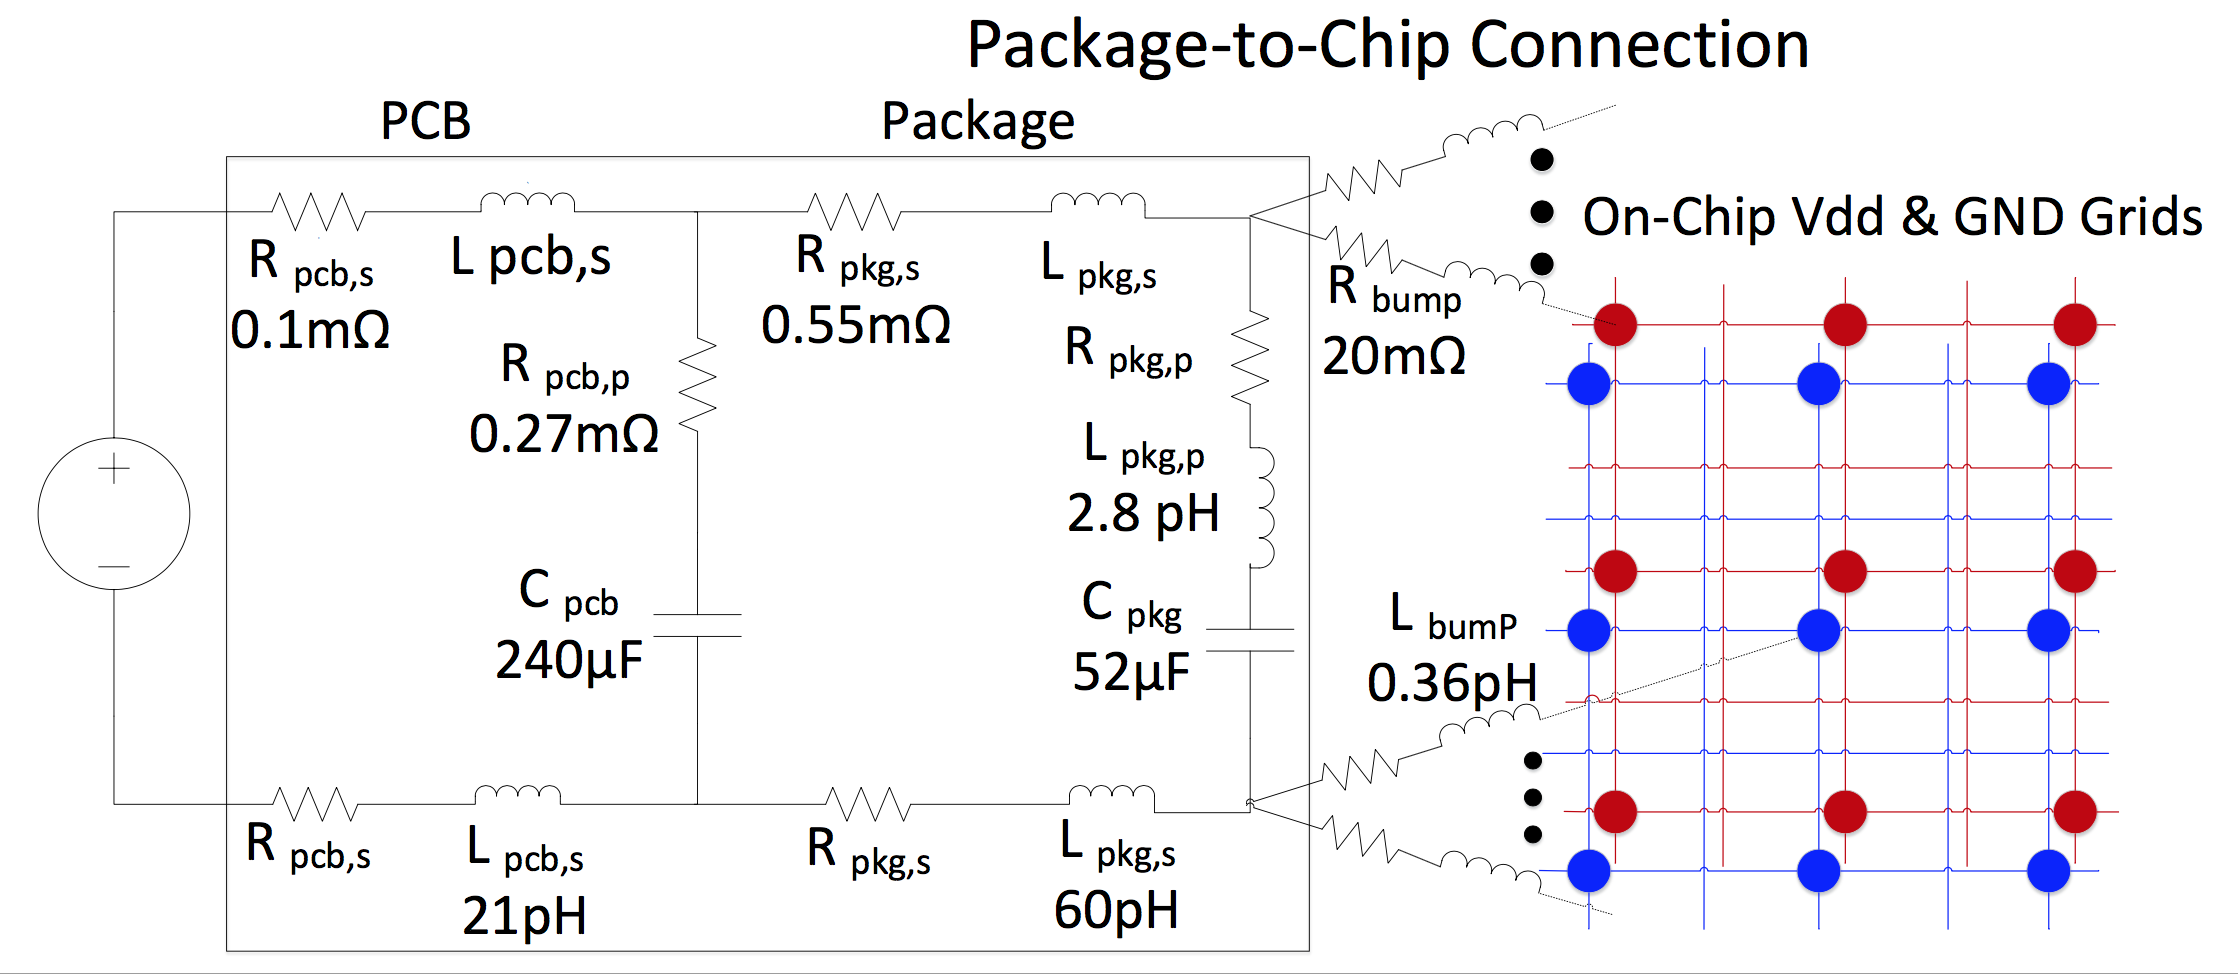
\includegraphics[trim=0 0 0 0,clip,width=0.8\linewidth]{graphs/pdn-model.png}
  \caption{An electrical model of the power delivery path from the voltage regulator module (VRM) to on-chip transistors. Impedance of different types exist on this path because of the electrical parasitics on the motherboard as well as inside the package. IR drop and the L$di/dt$ effect are caused by these parasitics.}
  \label{fig:pdn-model}
\end{figure*}

The supply voltage delivered to the CMOS transistors has lots of noise because the path from the source of voltage supply to the end transistors has lots of parasitics. Typically, the power supply subsystem can be modeled as four parts: the voltage regulator module, electrical parasitics on the printed circuit board, electrical parasitics at the package contact points, and on-die power delivery network. Each part has its own resistive, capacitive, and inductive parasitics that impede the transmission of voltage. These parasitics exist because the power delivery subsystem is made of real, physical materials - on-chip and off-chip wires have resistance even the magnitude can be small, wires can form loops by chance and create inductive impedance, the alignment between wires and the added decoupling capacitors create capacitance, etc.

Resistive parasitics cause supply voltage's IR drop following Ohm's law. Higher power causes higher IR drop. Inductive and capacitive parasitics further worsen supply voltage with the $di/dt$ effects. $di/dt$ effect happens when there is rapid change in the current draw, or power consumption of the transistors. $di/dt$ effect is happens rapidly, typically over tens of cycles, yet very rarely, making it hard to tract and especially dangerous. The combined IR drop and $di/dt$ effects make the supply voltage experienced by transistors very noisy. This adds uncertainty to the speed of microprocessor pipeline circuit. Therefore, timing margin, must be added to tolerate various voltage variation effects.

\paragraph{Process variation} is another source of uncertainty in circuit performance. Unlike temperature and voltage variation which change dynamically during runtime, process variation is a static effect that is formed during chip's manufacturing process, i.e., lithography. During lithography, noise can occur because the lithography instruments cannot perfectly control the various lithography steps, such as etching and doping. Wire width, transistor gate width and length can be etched with noise. Dopant density can deviate from the ideal density level. All these effects make transistor and wire's performance deviate from the ideal case, and make the speed of different transistors and wires differ. A microprocessor's performance is determined by the slowest part of the chip. The result is that faster circuits are forced to have some amount of timing margin because it is synchronized using the same clock as the slow circuits. We leave the study of timing margin caused by process variation to future work.

\paragraph{Other noisy effects} such as transistor aging, processor testing inaccuracy also contribute to pipeline circuit timing uncertainty. However, these effects' intensity is not as strong as temperature, voltage, and process variation aforementioned, and the condition for it to occur is too extreme. For this reason, we leave out these effects in this proposal and focus on voltage, temperature and process variation.

\subsection{The Need for Active Timing Margin and Its Management}
\label{sec:motivation:energy}

Traditionally, timing margin is fixed during chip design stage, the process of which follows a \textit{worst-case} design approach. In other words, the amount of timing margin must be able to tolerate the most extreme conditions that slow down microprocessor circuits, such as very heavy $di/dt$ voltage droops, very large IR drop caused by high power workloads, and unusual operating temperature that degrade transistor performance. The aggregate corner case of all effects determine how much timing margin is added to the chip.

The worst-case design approach described above is straightforward and easy to implement. Its design complexity is very low - simply raising voltage by some guardband value. It is also very robust in that all the worst-case conditions are tested and protected, so any timing uncertainty caused by any workload load condition should be tolerated because workload-induced uncertainty can be no worse than the hand-tuned worst-case condition. For years the worst-case timing margin approach has been the adopted and the down side of it has not drawn too much attention in microprocessor design and management because its voltage overhead is not as significant as other architecture performance or power issues. Yet, as various microarchitecture approach develops towards maturity and semiconductor technology scales to its limit, the research community is realizing that this static timing margin has become one of the golden opportunities that can be leveraged to squeeze power efficiency out of the underlying chip.

The main problem of the worst-case timing margin approach is that it is a static mechanism and overprovisions timing margin/voltage guardband resource most of the time. As an example, measurement on GPUs shows that most real-world programs do not need the full amount of voltage guardband. The reason is that the timing margin decided based on worst-case conditions are far different from the typical operating environments - workloads do not create extremely high or low temperature most of the time, nor do they invoke rapidly changing power variations often. These extreme conditions can only be met by specially built stress workloads like power and voltage virus programs, which involves non-trivial systematic design effort~\cite{kim2012audit,bertran2014voltage,bertran2012systematic}.

Real-world workloads often switch between different phases, and different phases may utilize the timing margin in very different manners. A program may enter a power hungry phase for a while, which induces heavy IR drop and raises chip temperature, and ultimately slows down transistors and consumes the timing margin heavily. After the computing in this phase is finished, the same program may enter a low power IO phase where circuit timing delay is small because of the low power, low IR drop, and mediate temperature levels. In this phase, timing margin is mostly wasted. The static, worst-case timing margin approach ignores workload dynamism and only targets the extreme situations, leaving timing margin unused and wasted most of the time. 

To work around the inefficiency of the worst-case static margin approach, timing margin must dynamically track workload behavior, check when workloads need timing margin, and provision it just-in-time. When workloads do not need high timing margin, voltage can be tuned down or frequency can be tuned up to save power or boost performance as illustrated in \Fig{fig:adaptive-margin}. This is the principle of \textit{active timing margin}. Figure xyz illustrates this idea with an $di/dt$ effect.

\begin{figure}[t!]
\captionsetup[subfloat]{width=0.4\textwidth}
\centering 
\subfloat[Static timing margin tolerates worst-case $di/dt$ effect with fixed low frequency.]
{
  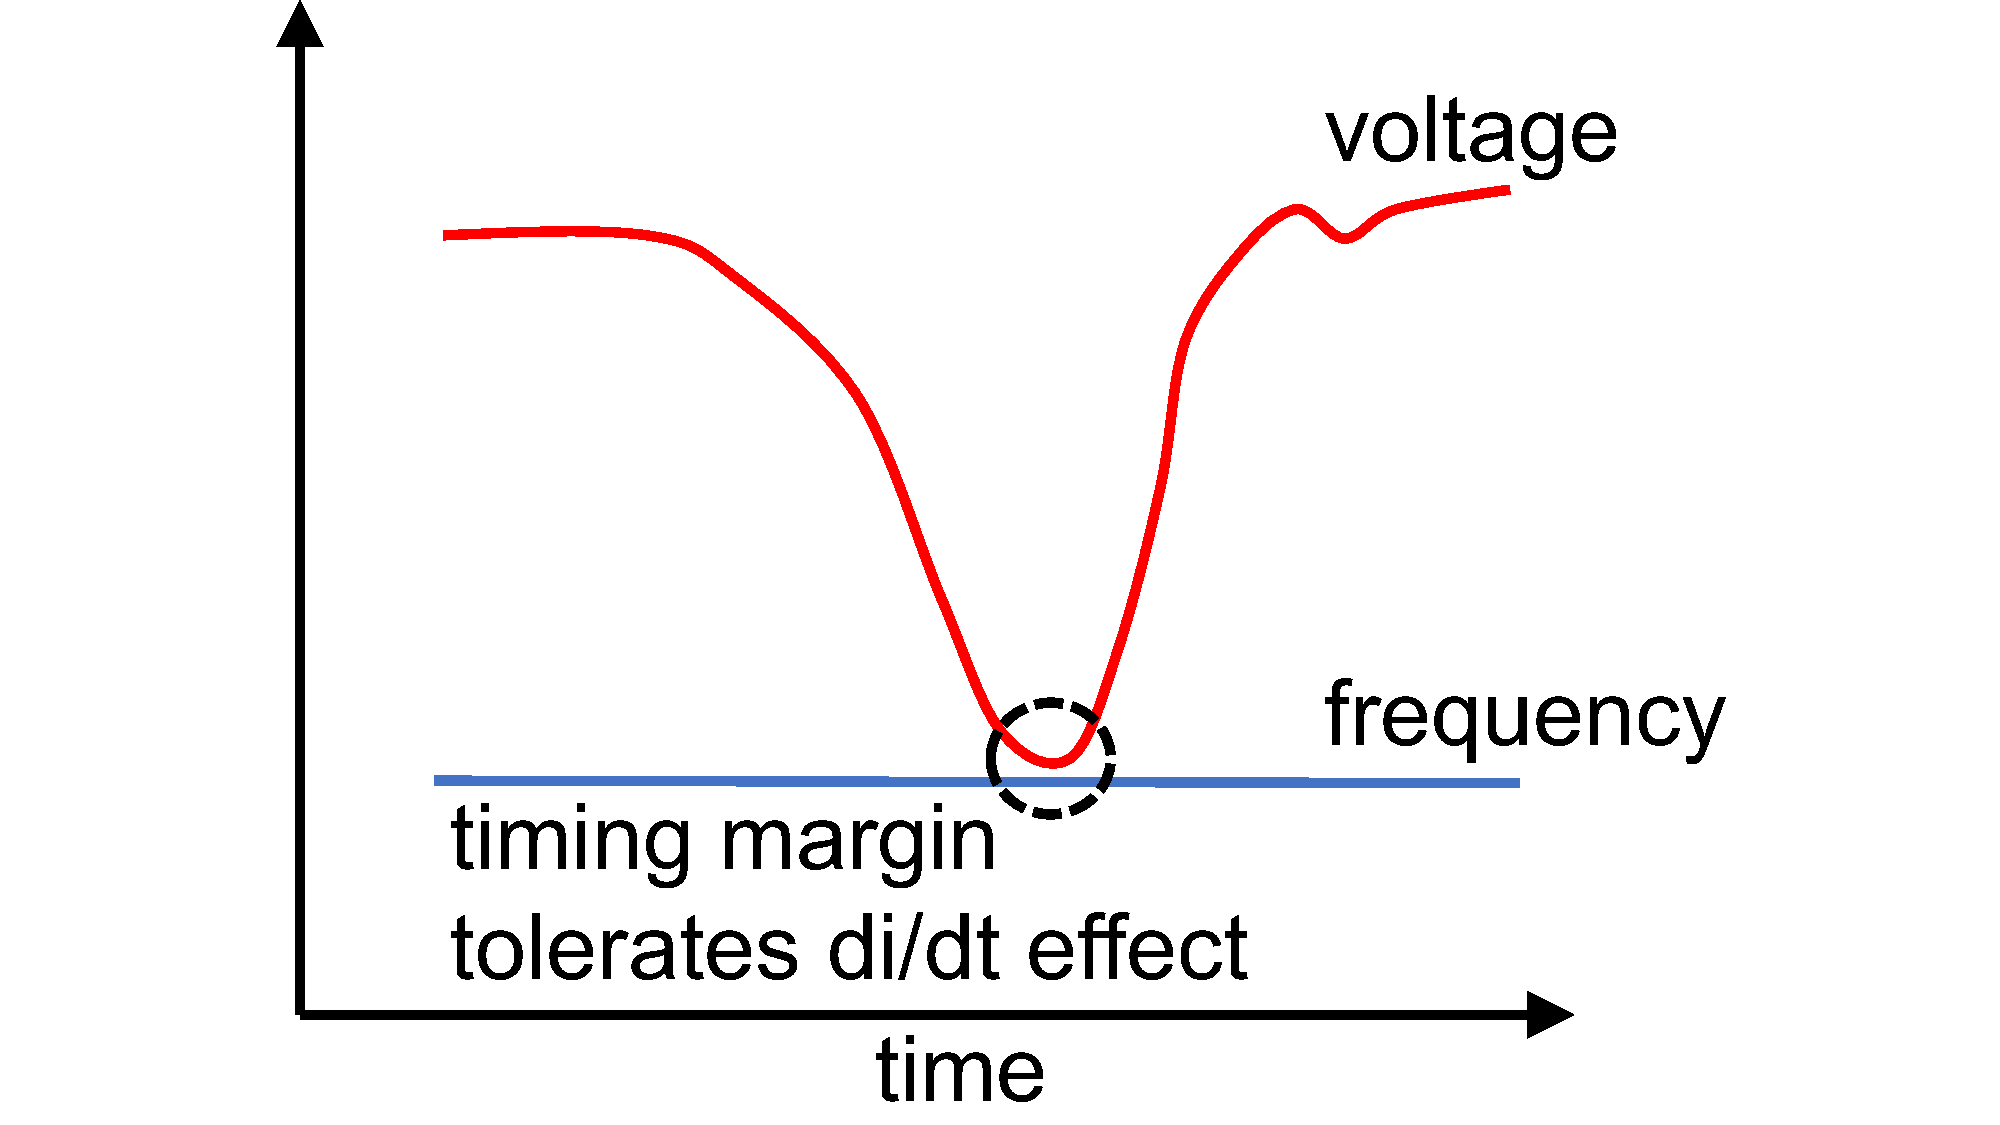
\includegraphics[trim=0 0 0 0,clip,width=0.47\linewidth]{graphs/didt-diagram1.pdf}
  \label{fig:didt-diagram1}
}
\subfloat[Active timing margin tolerates $di/dt$ effect by making frequency track voltage variation.] 
{
  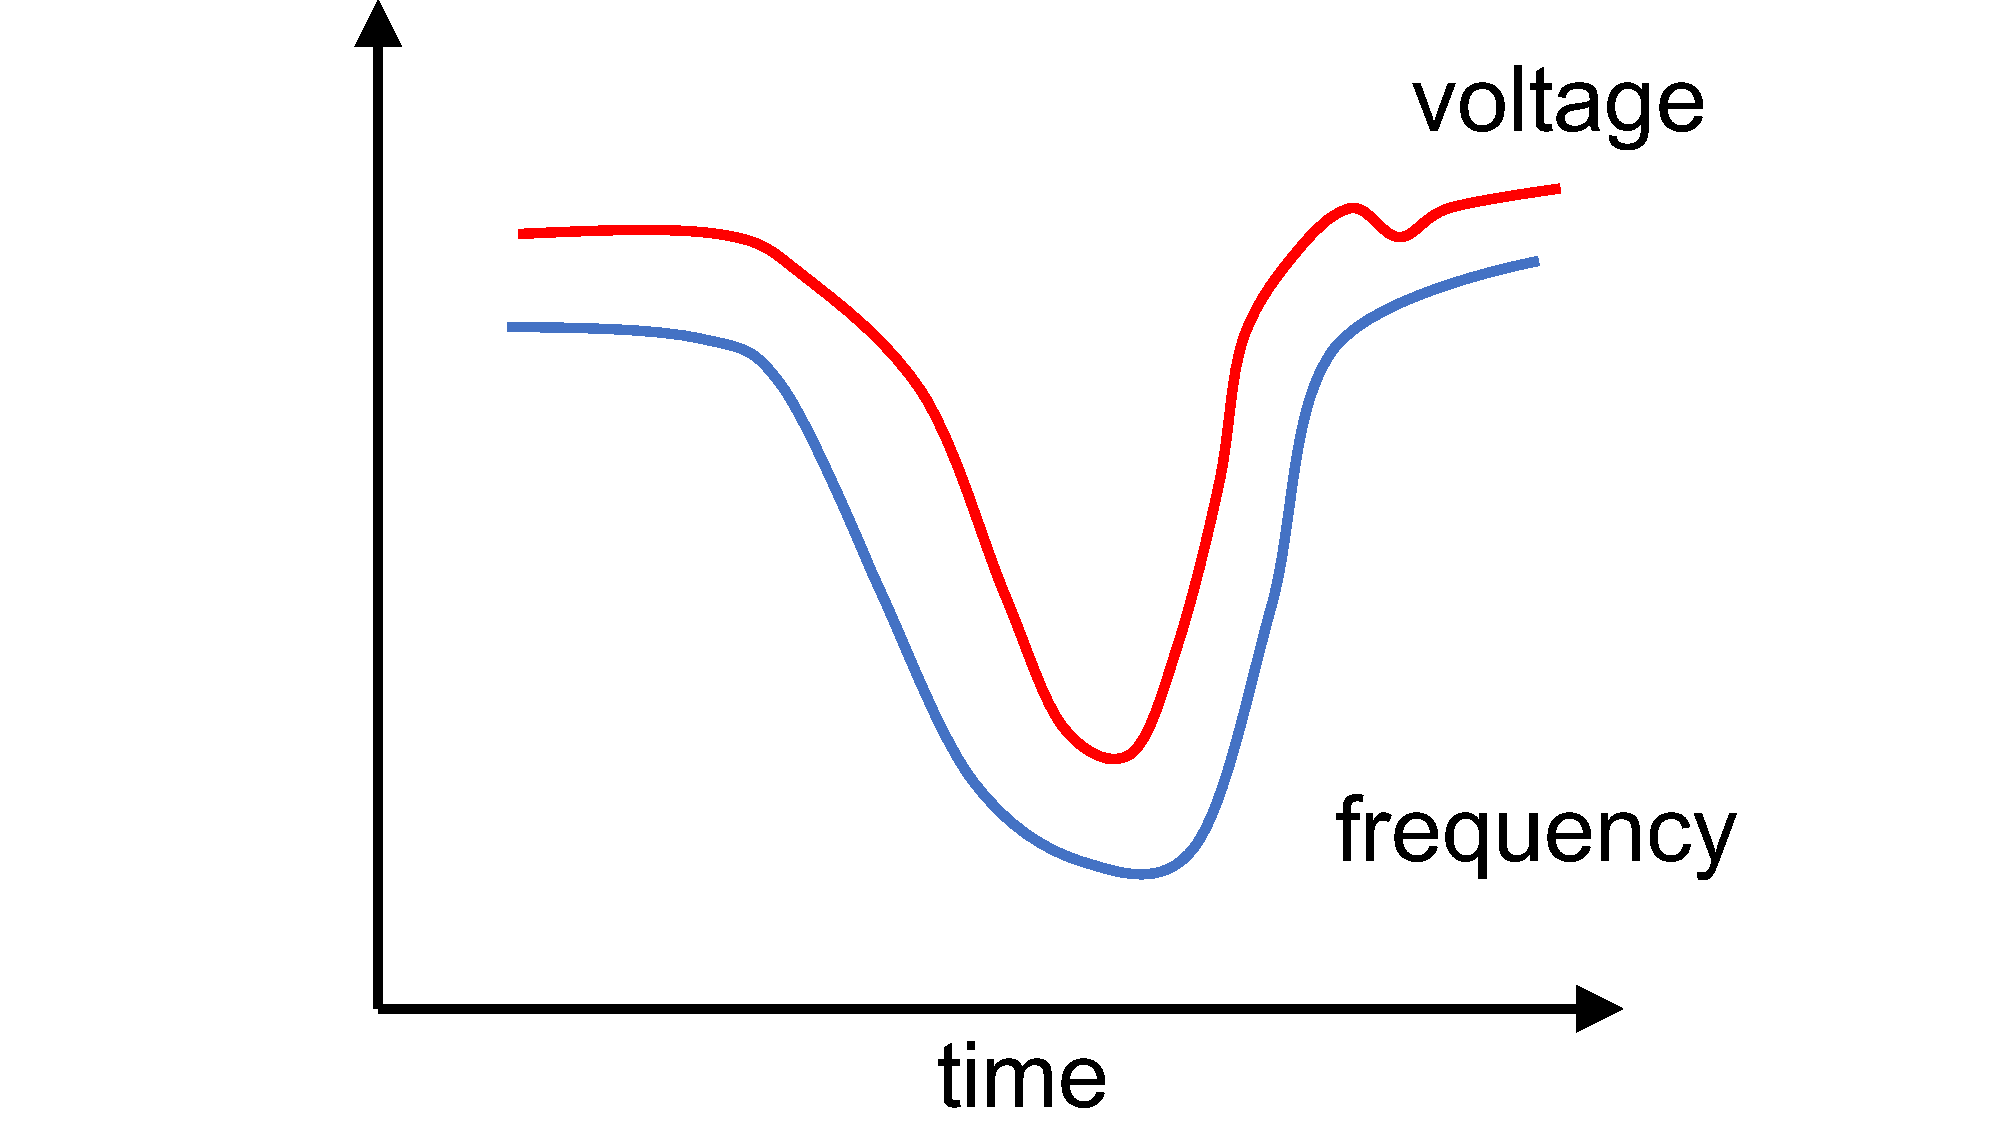
\includegraphics[trim=0 0 0 0,clip,width=0.47\linewidth]{graphs/didt-diagram2.pdf}
  \label{fig:didt-diagram2}
}
\caption{Active timing margin protects $di/dt$ effect by making frequency/clock cycle track supply voltage, which improves performance and reduces timing margin wastage.}
\vspace{-0.2in}
\end{figure}

In Figure \Fig{fig:didt-diagram1}, a heavy voltage droop caused by strong $di/dt$ effect slows down circuits, and necessitates some amount of timing margin to protect against it. The static margin does tolerate the $di/dt$ effect with a fixed, low frequency. However, only small voltage ripple occurs on the power delivery network when heavy $di/dt$ effect is not in place. During these periods, large timing margin is not needed, yet the static approach still provisions the timing margin set by the worst case, wasting a lot of performance under the same voltage. 

In \Fig{fig:didt-diagram2}, active timing margin dynamically adjust clock frequency to match the magnitude of voltage variation. When the $di/dt$ effect occurs, clock frequency ramps down quickly to provide the need timing margin. When there's no $di/dt$ effect, clock frequency stays at a higher level to reclaims the unused timing margin. Overall, the system enjoys higher performance.

Active timing margin bases itself on sensory detection of how emergent, or how much timing margin is used, and dynamically adjusts the amount of timing margin to match workload's need. When timing margin is used heavy, such as the case of strong IR drop, strong $di/dt$ effect, or on a core made of slow transistors, timing margin is added to provide extra space for safety. When timing margin is not used much, such as a light load workload phase, timing margin is shrunk to enhance efficiency. 

Along this line, we device active timing margin mechanism if solution corresponding to a particular effect does not exist yet, and explore active timing margin's implications for architecture design and system operation. We inspect possible ways to assist active timing margin to maximize its potential power efficiency benefits, and show that architecture and software cooperations are as important as implementing active timing margin itself to unlock the full opportunity hidden in timing margin.

%To work around the overprovisioning problem, researchers have explored various ways to shrink timing margin and still providing reliability guarantee. Example techniques include predicting emergency timing cases using instruction sequence, aggressively shrinking timing margin and relying on roll-back mechanisms, and using shadow latches to serve as ``error detection code''. These techniques are illuminating in that they point to the direction of first understanding what causes sever timing uncertainty cases, then devising techniques to act upon these cases correspondingly. However, these techniques, till this date, are still not widely practical because of their inherent design complexity issues. 
%Active timing margin does not need roll back mechanism in principle because it is not aggressive to the level that allows faults to occur. For this reason, the microarchitecture design overhead is small.
